\documentclass[aspectratio=1610]{beamer}

\usetheme{unnslides}
\usefonttheme{professionalfonts}

\usepackage{listings}
\usepackage{graphicx}
\usepackage{caption}
\usepackage{cmbright}
\usepackage{fontspec}
\usepackage{unicode-math}
\usepackage{amsfonts}
\usepackage{subfig}
\usepackage{tikz}

\captionsetup[subfigure]{labelformat=empty}
\captionsetup[figure]{labelformat=empty}

\setromanfont{CMU Serif}
%\setsansfont{CMU Sans Serif}
\setmathfont{Latin Modern Math}
\setlength{\tabcolsep}{1pt}

\usepackage{polyglossia}
%\setbeamertemplate{itemize item}{\color{black}$\blacktriangleright$}

\DeclareMathOperator*{\argmax}{arg\,max}
\DeclareMathOperator*{\argmin}{arg\,min}
\DeclareMathOperator{\sign}{sign}
\DeclareMathOperator{\re}{Re}

\graphicspath{ {../pictures/}{img/} }
%set pages numeration
%\setbeamertemplate{footline}[frame number]
%\setlength\abovecaptionskip{-3pt}

\addtobeamertemplate{navigation symbols}{}{%
    \usebeamerfont{footline}%
    \usebeamercolor[fg]{footline}%
    \hspace{1em}%
    \insertframenumber
}
\setbeamertemplate{headline}{}

\title{Comparison of Dimensionality Reduction Schemes for Parallel Global Optimization Algorithms}
\author{\textbf{Konstantin~Barkalov}, \textbf{Vladislav~Sovrasov} and \textbf{Ilya~Lebedev}}
\institute{Lobachevsky State University of Nizhni Novgorod}
\date{}

\begin{document}
\begin{frame}[noframenumbering,plain]
\titlepage
\end{frame}

\begin{frame}
  \frametitle{Problem statement}
  \begin{columns}
    \begin{column}{0.5\textwidth}
      \begin{displaymath}
        \begin{array}{cr}\\
          \varphi(y^*)=\min\{\varphi(y):y\in D\}, \\
          D=\{y\in \mathbb{R}^N:a_i\leq y_i\leq{b_i}, 1\leq{i}\leq{N}\}
        \end{array}
      \end{displaymath}
      \(\varphi(y)\) is multiextremal objective function, which satisfies the Lipschitz condition:
      \begin{displaymath}
        |\varphi(y_1)-\varphi(y_2)|\leq L\Vert y_1-y_2\Vert,y_1,y_2\in D,
      \end{displaymath}
      where \(L>0\) is the Lipschitz constant, and \(||\cdot||\) denotes \(l_2\) norm in \(\mathbb{R}^N\)
      space.
    \end{column}
    \begin{column}{0.5\textwidth}
      \centerline{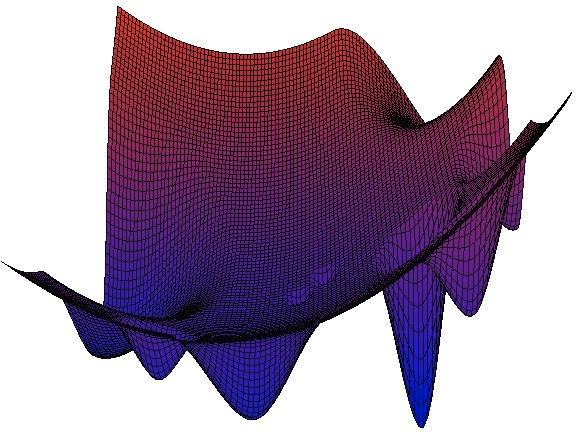
\includegraphics[width=0.9\textwidth]{img/gkls.png}}
    \end{column}
  \end{columns}
\end{frame}

\begin{frame}
  \begin{center}


  \frametitle{Dimension reduction}
  Peano-type curve \(y(x)\) allows to reduce the dimension of the original problem:
  \begin{gather}
    \lbrace y\in \mathbb{R}^N:-2^{-1}\leqslant y_i\leqslant 2^{-1},1\leqslant i\leqslant N\rbrace=\{y(x):0\leqslant x\leqslant 1\} \nonumber \\
    \min\{f(y): y\in D\}=\min\{f(y(x)): x\in [0,1]\} \nonumber
  \end{gather}
  \(y(x)\) is non-smooth function which continuously maps the segment \([0,1]\) to the hypercube \(D\).
  \begin{figure}[ht]
    \vspace*{-0.5cm}
    \subfloat{{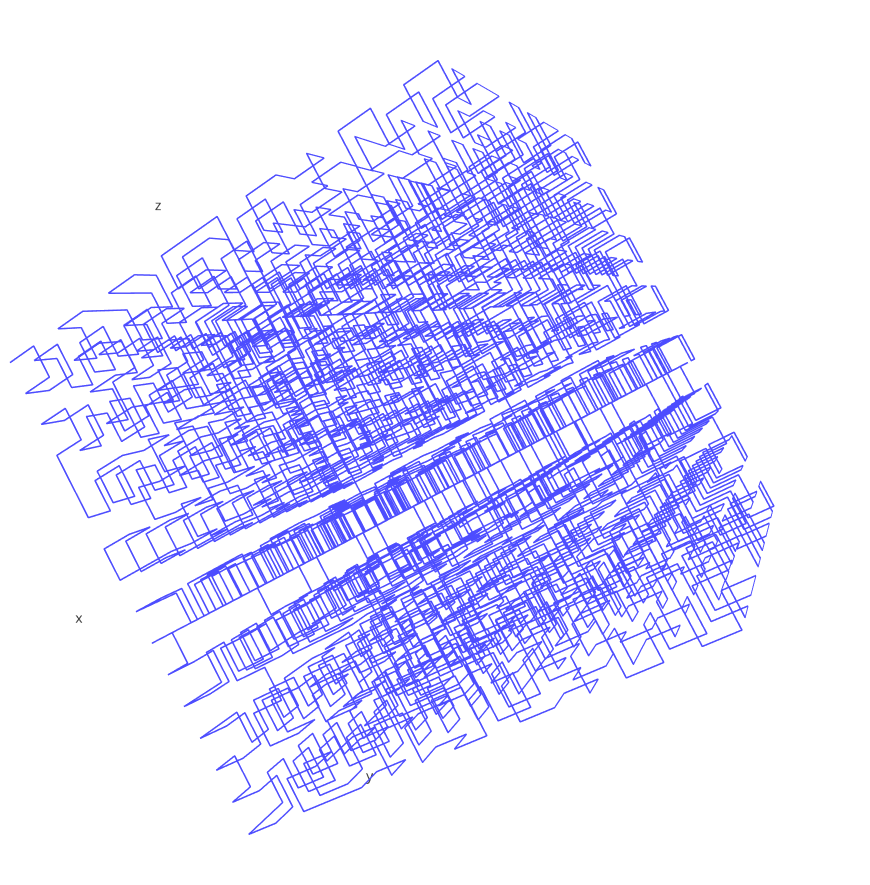
\includegraphics[width=.35\textwidth]{peano3d.png} }}
    \subfloat{{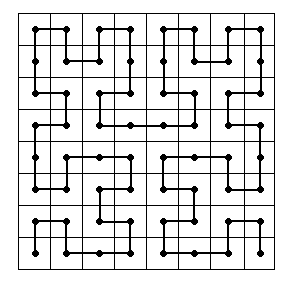
\includegraphics[width=.35\textwidth]{peano2d.png} }}
  \end{figure}
\end{center}
\end{frame}

\begin{frame}
  \frametitle{Properties of the reduced problem}
  After applying the Peano-type evolvent \(\varphi(y(x))\) satisfies the uniform H{\"o}lder condition:
  \begin{displaymath}
    |\varphi(y(x_1))-\varphi(y(x_2))|\leq H{|x_1-x_2|}^{\frac{1}{N}}, x_1,x_2\in[0,1],
  \end{displaymath}
  \(\varphi(y(x))\) is non-smooth and has multiple local and \textbf{global} extremums even if \(\varphi(y)\) is unimodal.
  The latter problem is caused by loss of the information about \(N\)-d neighborhood after the transformation to the \(1\)-d space.

  \begin{figure}[ht]
    \begin{center}

    \vspace*{-0.5cm}
    \subfloat{\raisebox{.02\textheight}{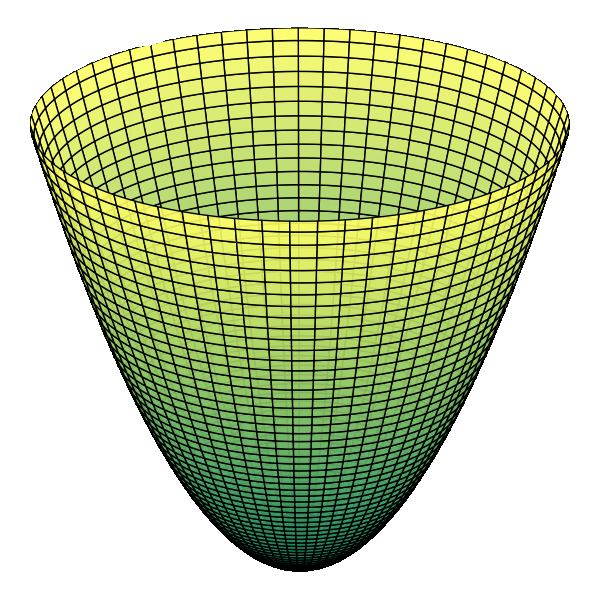
\includegraphics[width=.3\textwidth]{parabaloid.png}}}
    \subfloat{\raisebox{.2\textheight}{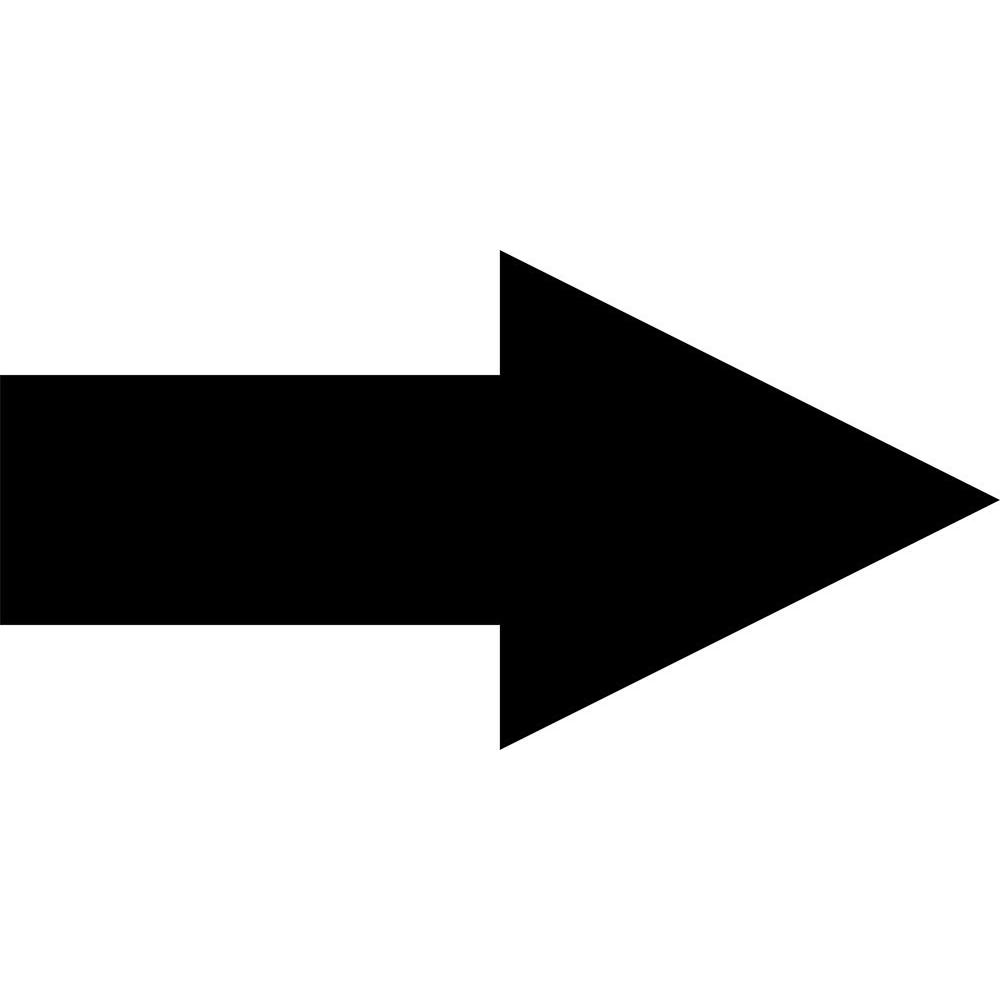
\includegraphics[width=.05\textwidth]{arrow.jpg}}}
    \subfloat{{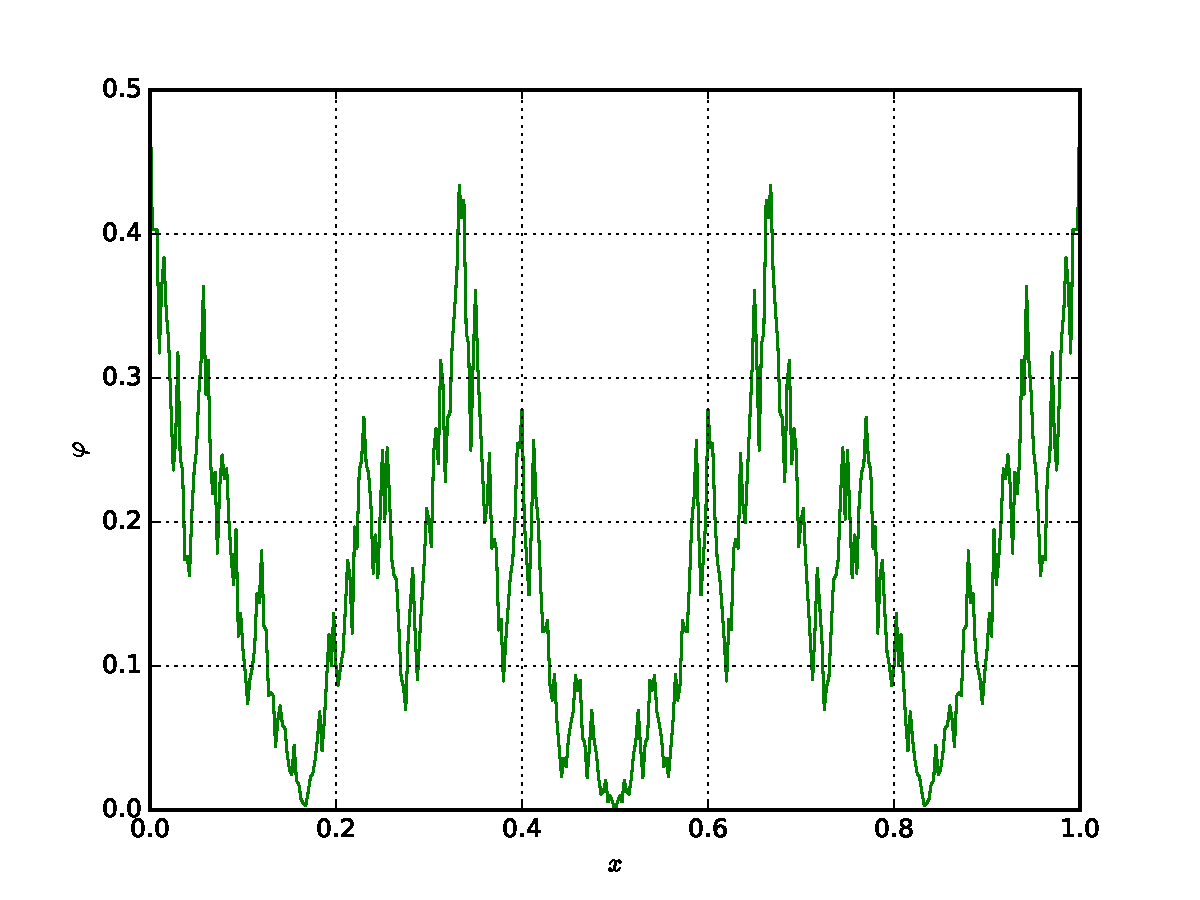
\includegraphics[width=.45\textwidth]{map_paraboloid.pdf}}}
  \end{center}
  \end{figure}
\end{frame}

\begin{frame}
  \frametitle{Non-univalent evolvent}
    One can try to recover all preimages of \(y\in\mathbb{R}^N\) and make optimization method aware of their existence\footnote{R.G. Strongin. Numerical Methods in Multiextremal Problems (in Russian), 1978}. This allows reducing the effect of growing amount of local minimas after dimension reduction.
    According to the theory of Peano-type curves, each \(N\)-d point could have up to \(2^N\) preimages. For large \(N\) such preimages mining would be expensive.
      \begin{figure}[ht]
        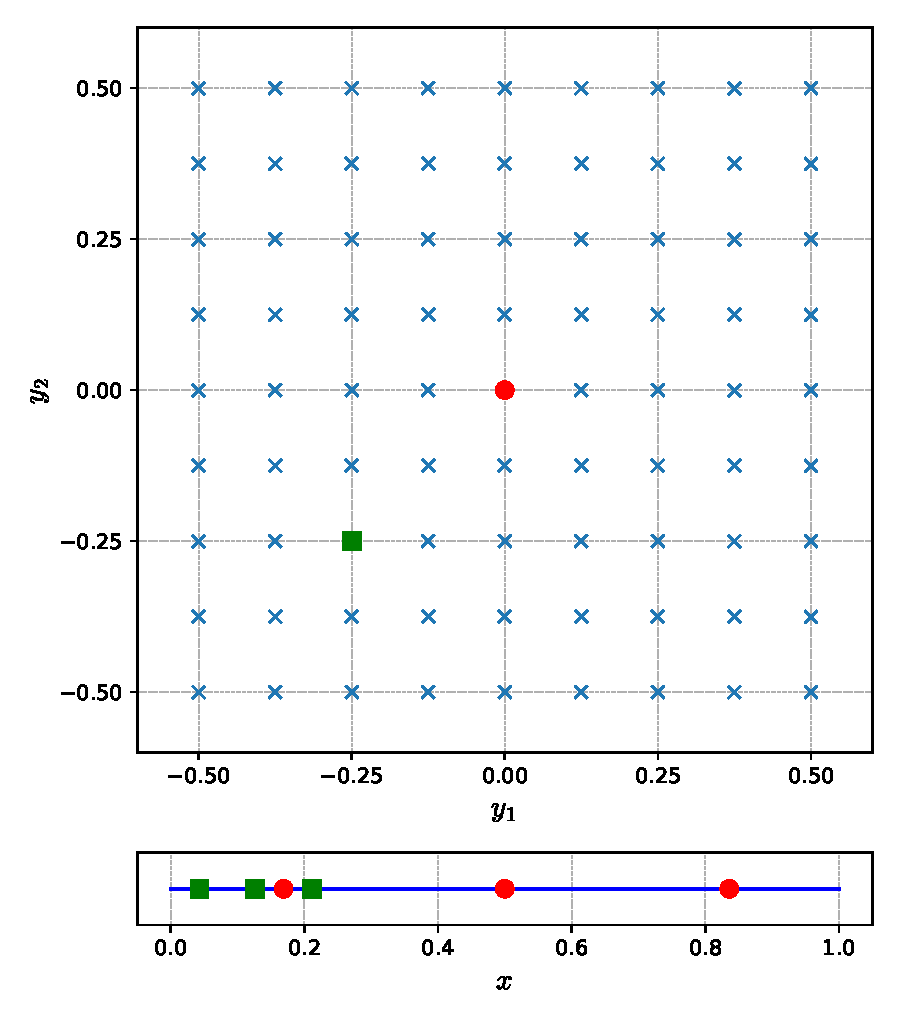
\includegraphics[width=.25\textwidth]{noninjective.pdf}
      \end{figure}
\end{frame}

\begin{frame}
  \frametitle{Shifted and rotated evolvents}
  To create a fixed amount of preimages one can use a pre-defined set of different evolvents. These evolvents could be shifted or rotated versions of the original one. Set of shifted evolvents\footnote{Strongin, R.G., Gergel, V.P., Barkalov, K.A. Parallel methods for global optimization problem
solving (in Russian), 2009} is theoretically proven to generate at least one pair of close preimages if images are close and it perform better than the set of rotated curves.
  \begin{figure}[ht]
    \subfloat{\raisebox{.0\textheight}{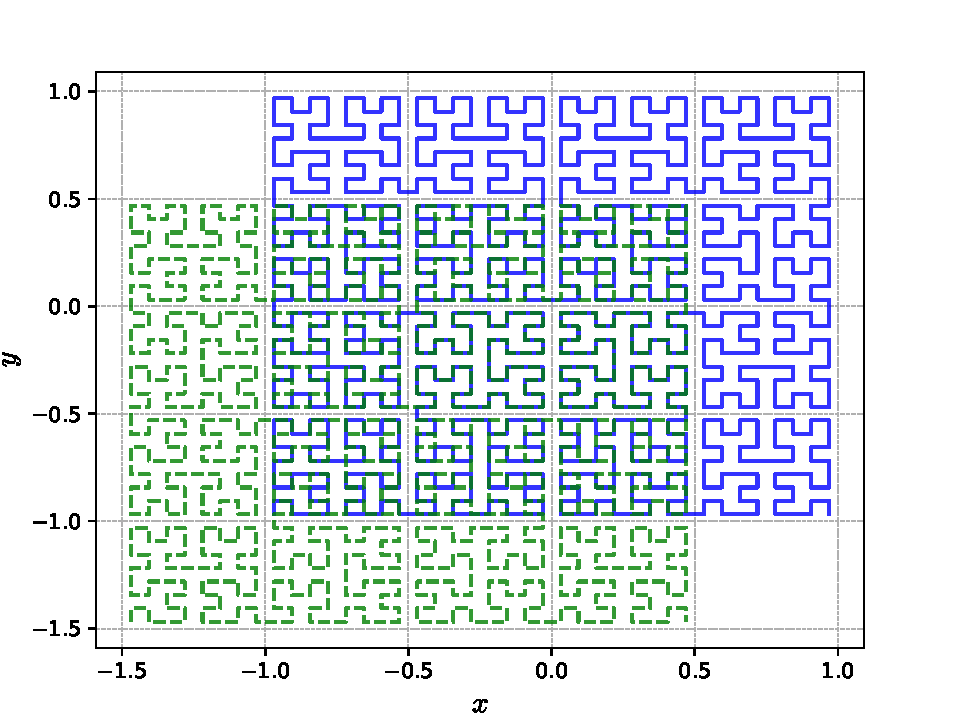
\includegraphics[width=.35\textwidth]{shifted.pdf} }}
    \subfloat{{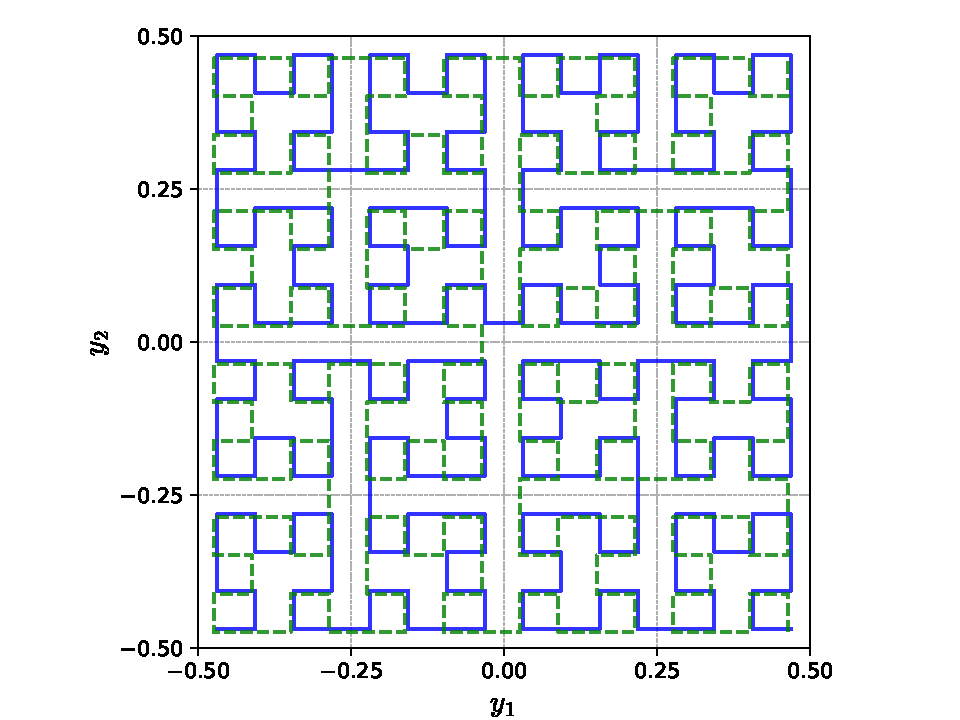
\includegraphics[width=.35\textwidth]{rotated.pdf} }}
  \end{figure}
\end{frame}

\begin{frame}
  \frametitle{Smooth evolvent}
  Smooth functions are more predictable for optimizer, so smooth approximation of the Peano-like \(y(x)\) curve could improve convergence rate \footnote{Goryachih, A. A class of smooth modification of space-filling curves for global optimization problems, NET 2016}.
  \begin{figure}[ht]
    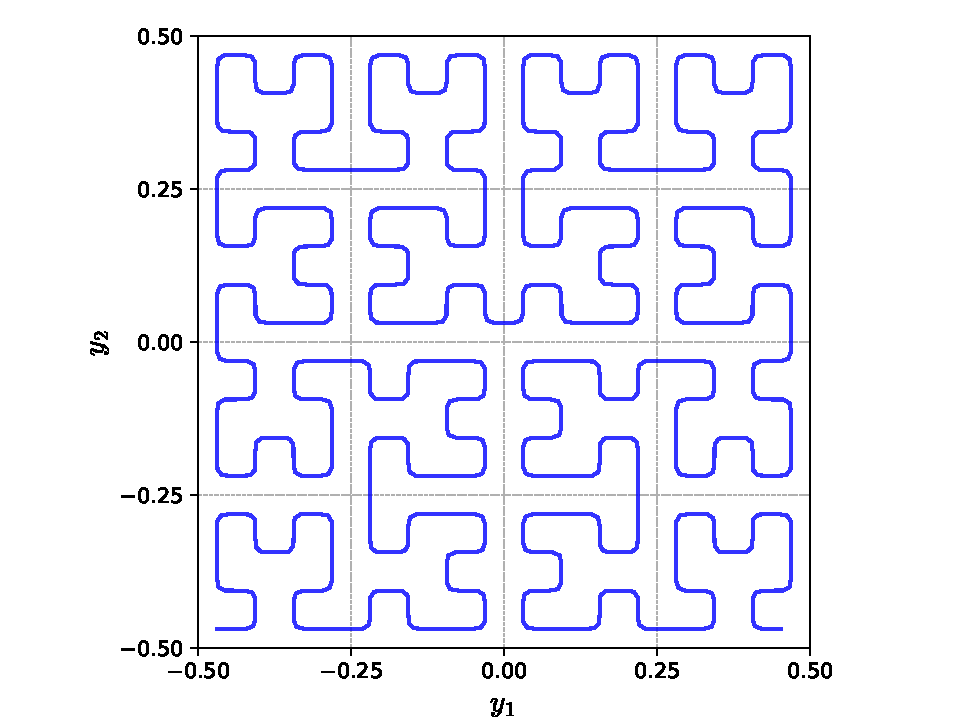
\includegraphics[width=0.45\textwidth]{smooth.pdf}
  \end{figure}

\end{frame}

\begin{frame}
  \frametitle{Basic parallel optimization method}
  Optimization method generates search sequence \(\{x_k\}\) and consists of the following steps:
  \begin{enumerate}
    \setlength{\itemindent}{.1in}
    \item[Step 1.] Sort the search information (one-dimensional points) in increasing order.
    \item[Step 2.] Compute the evolvent \(y(x^{k+j})\) and the function \(\varphi(y(x^{k+j}))\), \(j=\overline{1,p}\).
    \item[Step 3.] For each interval \((x_{i-1}, x_i)\) compute quantity \(R(i)\), called characteristic.
    \item[Step 4.] Choose \(p\) intervals \((x_{t_j-1}, x_{t_j})\) with the greatest characteristics and
    compute objective \(f(y(x^{k+j}))\) in points chosen using the decision rule \(d\):
    \begin{displaymath}
      x^{k+1+j}=d(t)\in (x_{t_j-1}, x_{t_j}),\:j=\overline{1,p}
    \end{displaymath}
    \item[Step 5.] If \(x_{t_j}-x_{t_j-1}<\varepsilon\) for one of \(j=\overline{1,p}\), stop the method.
  \end{enumerate}
  \textit{\footnotesize	{Detailed description: Strongin R.G., Sergeyev Ya.D.: Global optimization with non-convex constraints. Sequential and parallel algorithms (2000), Chapter 7}}
\end{frame}

\begin{frame}
  \frametitle{Parallel optimization method with multiple evolvents}
  Using the multiple mapping allows solving initial problem by parallel solving the problems
  \[
  \min\{\varphi(y^s(x)):x\in [0,1]\}, 1\leqslant s\leqslant S
  \]
  on a set of intervals $[0,1]$ by the index method. Each one-dimensional problem is solved on a
  separate processor. The trial results at the point \(x^k\) obtained for the problem being solved by
  particular processor are interpreted as the results of the trials in the rest problems (in the
  corresponding points \(x^{k_1},\dots,x^{k_S})\). In this approach, a trial at the point \(x^k \in
  [0,1]\) executed in the framework of the \(s\)-th problem, consists in the following sequence of
  operations:
  \begin{enumerate}
    \setlength{\itemindent}{.1in}
    \item[Step 1.] Determine the image \(y^k=y^s (x^k)\) for the evolvent \(y^s (x)\).
    \item[Step 2.] Inform the rest of processors about the start of the trial execution at the point \( y^k\) (the
    blocking of the point \(y^k\) ).
    \item[Step 3.] Determine the preimages \(x{}^{k_s}  \in [0,1], 1\leqslant s\leqslant S\), of the point \(y^k\) and interpret the
    trial executed at the point \(y^k \in D \) as the execution of the trials in the \(S\) points
    \(x{}^{k_1} ,\dots,x{}^{k_s} \)
    \item[Step 4.] Inform the rest of processors about the trial results at the point \(y^k\).
  \end{enumerate}
\end{frame}

\begin{frame}
  \frametitle{Test problems}
  \begin{columns}
    \begin{column}{0.5\textwidth}
      Generator GKLS was employed to construct the sets of test problems:
      \begin{displaymath}
        \begin{matrix}
          f(x)=
          \left\{
          \begin{matrix}
          C_i(x), x \in S_i, i\in 2,\dots ,m \\
          \Vert x-T \Vert^2 + t, x\not\in S_2,\dots,S_m
          \end{matrix} \right.
        \end{matrix}
      \end{displaymath}

      The generator allows to adjust:
      \begin{itemize}
        \item the number of local minimas;
        \item the size of the global minima attraction region;
        \item the space dimension.
      \end{itemize}
    \end{column}
    \begin{column}{0.5\textwidth}
      \centerline{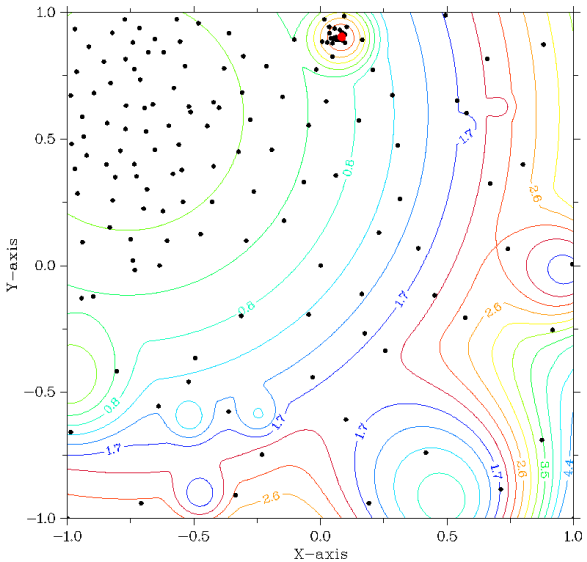
\includegraphics[width=0.9\textwidth]{gkls_color.png}}
    \end{column}
  \end{columns}
\end{frame}

\begin{frame}
  \frametitle{Evolvents comparison}
  \begin{figure}[ht]
    \hspace*{-0.9cm}
    \subfloat[Minimal \(r\)]{{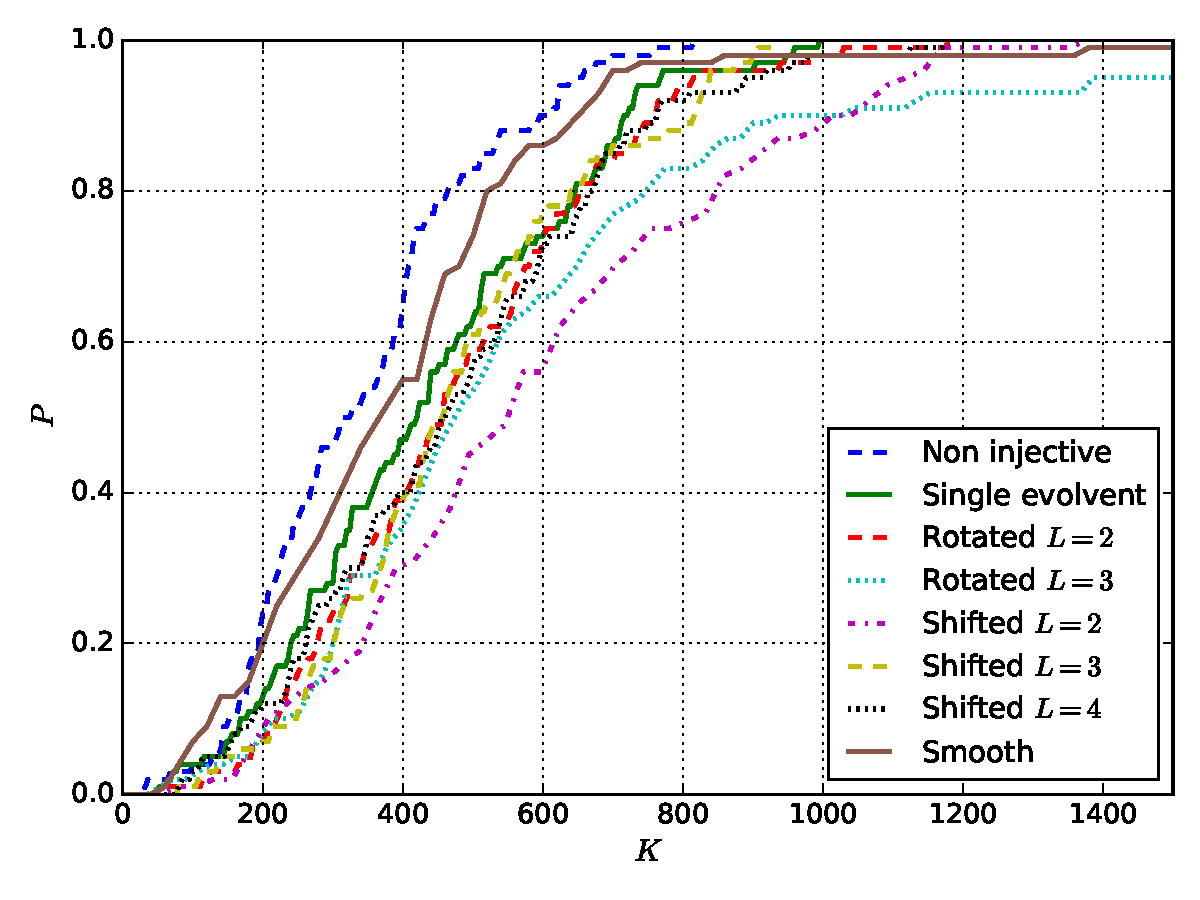
\includegraphics[width=.55\textwidth]{gklsS2d_opt_pt_op.pdf} }}
    \subfloat[\(r=5.0\)]{{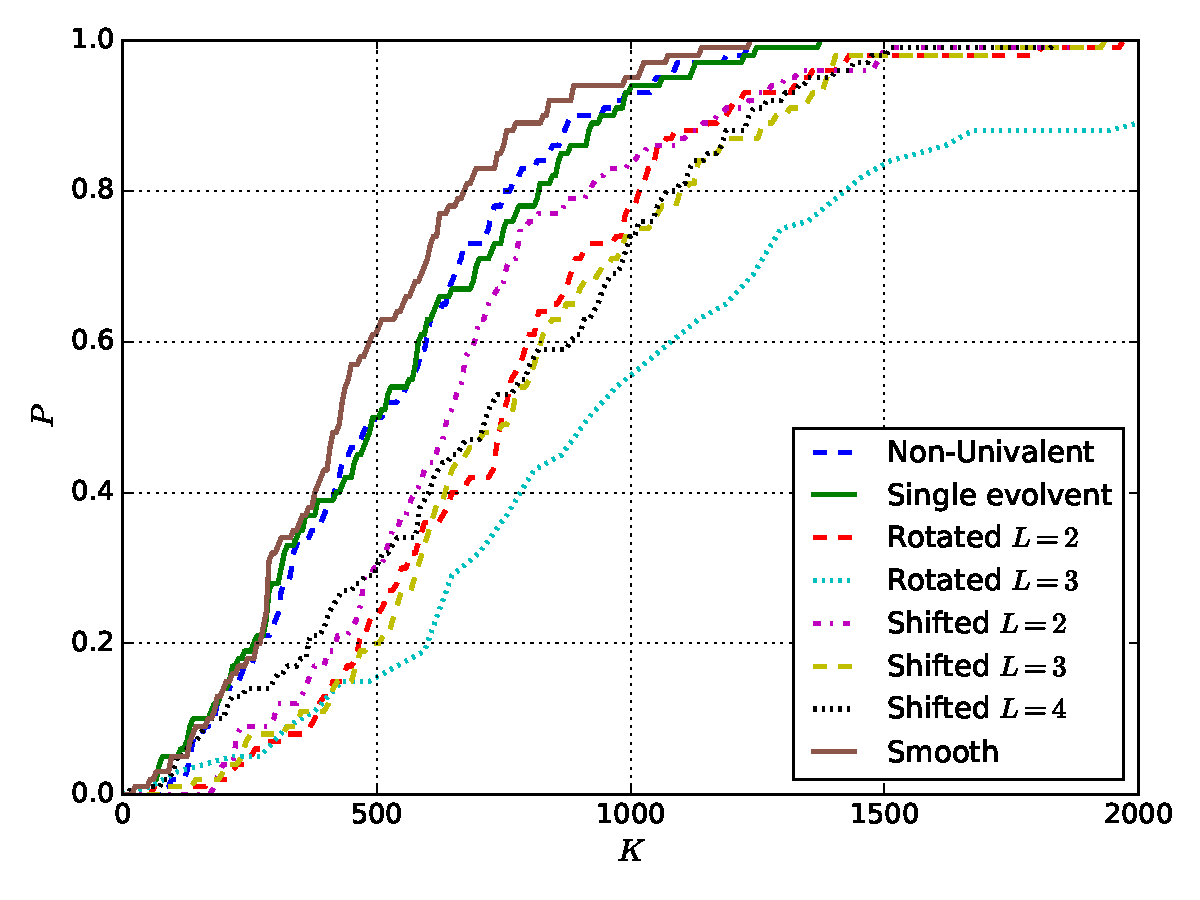
\includegraphics[width=.55\textwidth]{gklsS2d_same_r_opt_pt_op.pdf} }} \hspace*{4cm}
    \caption{Operating characteristics on GKLS 2d Simple class}
  \end{figure}
\end{frame}

\begin{frame}
  \frametitle{Evolvents comparison}
  \begin{figure}[ht]
    \hspace*{-0.9cm}
    \subfloat[Minimal \(r\)]{{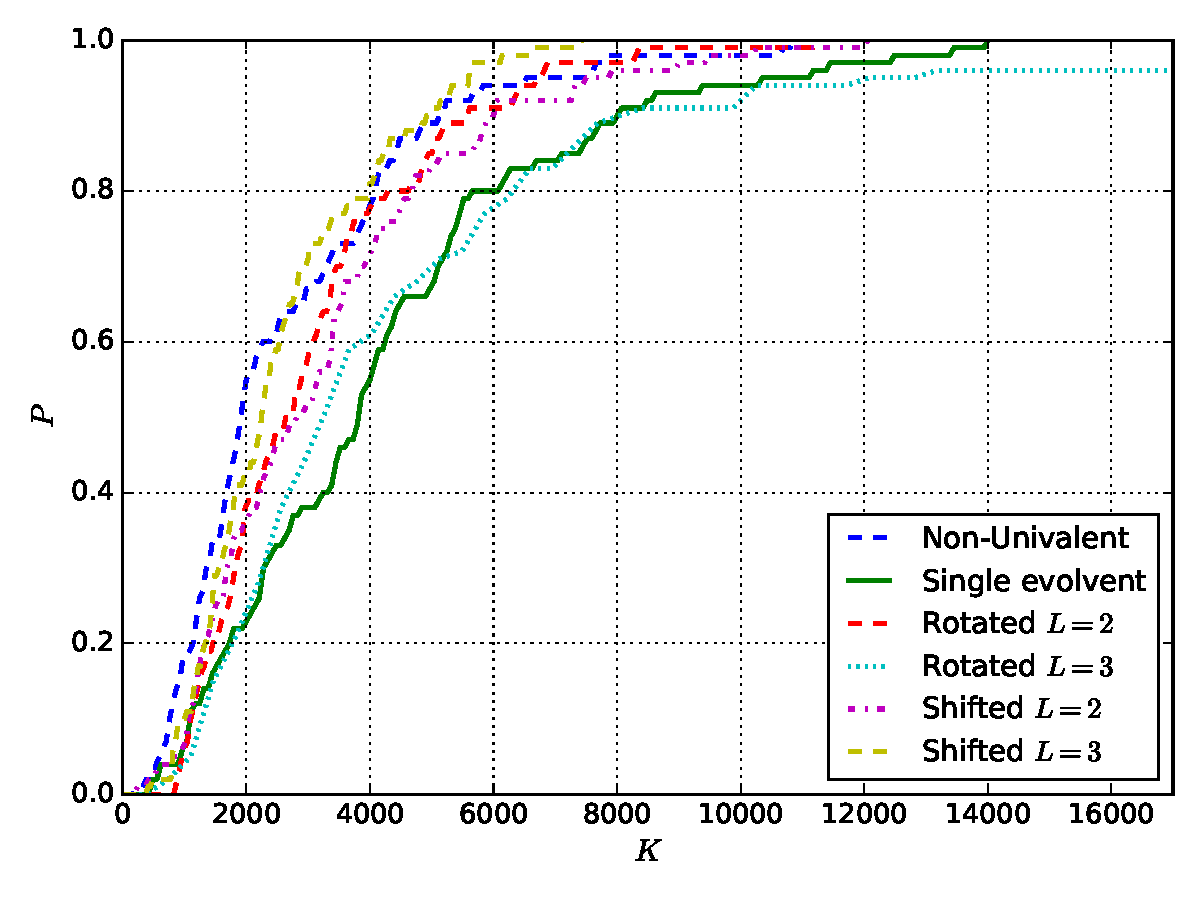
\includegraphics[width=.55\textwidth]{gklsS3d_opt_pt_op.pdf} }}
    \subfloat[\(r=4.5\)]{{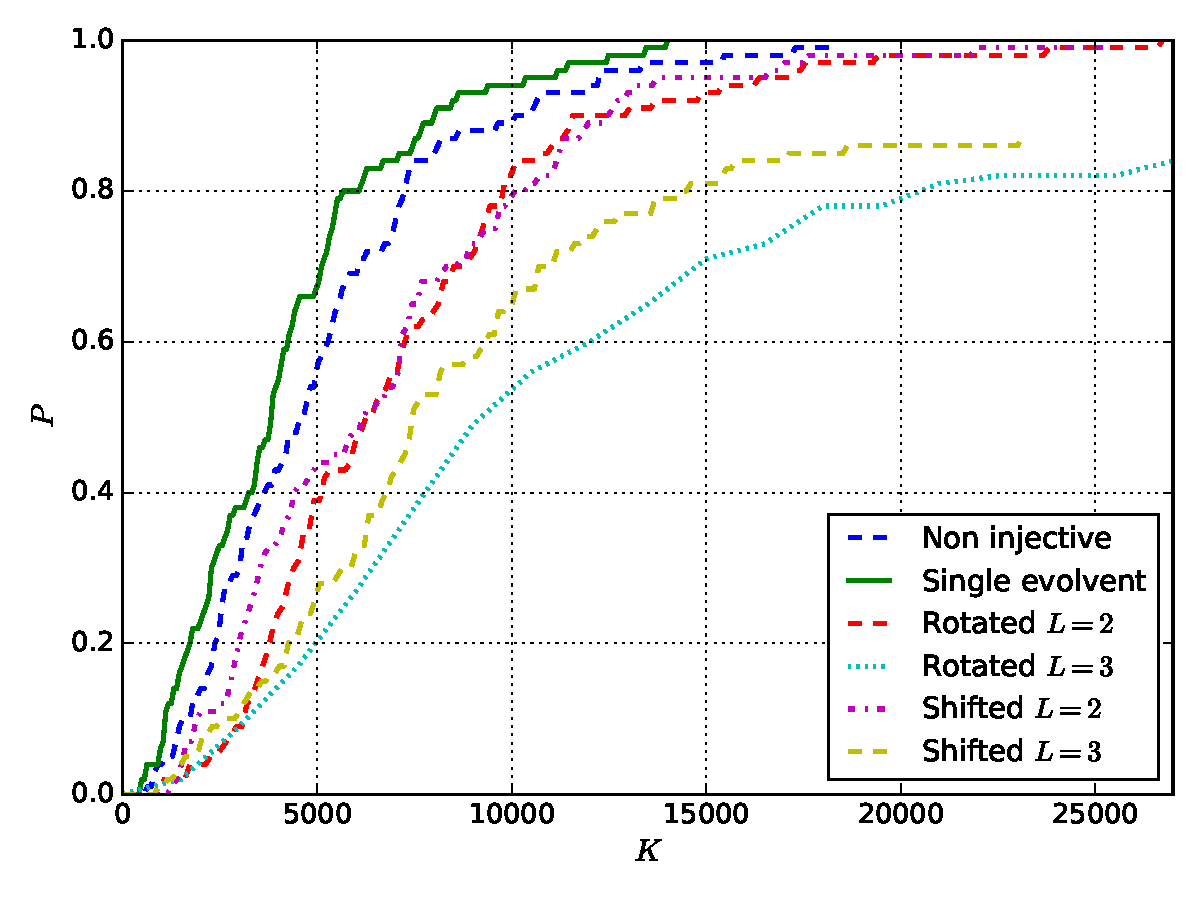
\includegraphics[width=.55\textwidth]{gklsS3d_same_r_opt_pt_op.pdf} }}
    \caption{Operating characteristics on GKLS 3d Simple class}
  \end{figure}
\end{frame}

\begin{frame}
  \frametitle{Choice of evolvent for the parallel algorithm}
  \begin{table}
  \begin{center}
  \caption{Averaged number of computations of \(g_0\) and of \(\varphi\) when solving the
  problems from GKLS 3d Simple class using the shifted evolvent}
    \begin{tabular}{|l|{c}|{c}|{c}|}
      \hline
    $L$ & $calc(g_0)$ & $calc(\varphi)$ & $\frac{calc(g_0)}{calc(\varphi)}$ ratio \\
    \hline
    2 & 96247.9  & 6840.14 & 14.07\\
    \hline
    3 & 153131.0 & 7702.82 & 19.88\\
    \hline
    \end{tabular}
    \label{tab:shifted_g0}
  \end{center}
  \end{table}
\end{frame}

\begin{frame}
  \frametitle{Results of applying the parallel algorithm}

  \begin{table}
    \centering
    \caption{Averaged numbers of iterations executed by the parallel algorithm for solving the test
  optimization problems}
    \label{tab:iterations}
    \begin{tabular}{cccccccc}
      \cline{3-8}\noalign{\smallskip}
      \multicolumn{2}{c}{  } & \textit{p} & \multicolumn{2}{c}{$N=4$} & &
  \multicolumn{2}{c}{$N=5$}   \\
      \noalign{\smallskip} \cline{4-5} \cline{7-8}  \noalign{\smallskip}
      \multicolumn{2}{c}{  } & & \textit{Simple} & \textit{Hard} & & \textit{Simple} &
  \textit{Hard}  \\
      \noalign{\smallskip}\hline
      I &
      \parbox{0.25\textwidth}{
      \begin{center}
      \textbf{1 cluster node}
      \end{center}		}
        & \textit{1} & 12167 & 25635 & & 20979 & 187353  \\
      &  & \textit{32} & 328 & 1268  & &   898 & 12208 \\
      \hline \noalign{\smallskip}
  II  & \textbf{4 cluster nodes}  %\multirow{3}{*}{}
    & \textit{1} & 25312 & 11103 & & 1472 & 17009 \\
  &   & \textit{32} & 64 &   913 & & 47 & 345 \\
      \noalign{\smallskip}\hline	\noalign{\smallskip}
  III & \textbf{8 cluster nodes} %\multirow{3}{*}{}
    & \textit{1}  & 810 & 4351 & & 868 & 5697  \\
  & & \textit{32} & 34  & 112  & & 35  & 868 \\
      \noalign{\smallskip}\hline
    \end{tabular}
  \end{table}

\end{frame}

\begin{frame}
  \frametitle{Results of applying the parallel algorithm}

  \begin{table}
    \centering
    \caption{Speedup of parallel computations executed by the parallel algorithm}
    \label{tab:speedup}
    \begin{tabular}{cccccccc}
      \cline{3-8}\noalign{\smallskip}
      \multicolumn{2}{c}{  } & \textit{p} & \multicolumn{2}{c}{$N=4$} & &
  \multicolumn{2}{c}{$N=5$}   \\
      \noalign{\smallskip} \cline{4-5} \cline{7-8}  \noalign{\smallskip}
      \multicolumn{2}{c}{  } & & \textit{Simple} & \textit{Hard} & & \textit{Simple} &
  \textit{Hard}  \\
      \noalign{\smallskip}\hline
      I &
      \parbox{0.25\textwidth}{
      \begin{center}
      \textbf{1 cluster node}
      \end{center}		}
      & \textit{1}   & 12167(10.58s) & 25635(22.26s) & & 20979(22.78s) & 187353(205.83s)  \\
    &  & \textit{32} & 37.1(18.03) & 20.2(8.55)  & &  23.3(8.77) & 15.4(9.68) \\
    \hline \noalign{\smallskip}
  II  & \textbf{4 cluster nodes}  %\multirow{3}{*}{}
  & \textit{1} &        0.5(0.33) & 2.3(0.86)  & & 14.3(6.61) & 11.0(6.06) \\
  &   & \textit{32} & 190.1(9.59) & 28.1(1.08) & & 446.4(19.79) & 543.0(43.60) \\
    \noalign{\smallskip}\hline	\noalign{\smallskip}
  III & \textbf{8 cluster nodes} %\multirow{3}{*}{}
  & \textit{1}    & 15.0(6.05)  & 5.9(2.36)   & & 24.2(17.56)  & 32.9(24.87)  \\
  & & \textit{32} & 357.9(2.36) & 228.9(2.64) & & 582.8(20.96) & 793.0(33.89) \\
      \noalign{\smallskip}\hline
    \end{tabular}
  \end{table}

\end{frame}

\begin{frame}
  \frametitle{Conclusions}
    %Already done:
    \begin{itemize}
      \item the smooth evolvent and the non-univalent one demonstrate the best result in the problems of small dimensionality and can be applied successfully in solving the problems with the computational costly objective functions.
      \item the shifted evolvents introduce large overhead costs on the execution of the method due to the requirement to adding an auxiliary constraint. About 95\% of iterations are overhead to fight the auxiliary constraint.
      \item rotated evolvents perform almost the same as the shifted ones but without overhead.
      \item parallel optimization method shows up to 33x speedup on hard \(5d\) problems when using a set of rotated evolvents.
    \end{itemize}
    %Future work:
    %\begin{itemize}
    %  \item
    %\end{itemize}
\end{frame}

\begin{frame}{{}}
  \frametitle{Q\&A}
  \begin{center}
    \Large{Contacts:}
\vspace{0.5cm}

    sovrasov.vlad@gmail.com

    https://github.com/sovrasov
  \end{center}
\end{frame}

\end{document}
